\section{Introduction}
\label{sec:introduction}

Modern software applications are complex and diverse in nature. They come in 
various forms ranging from large web-based systems that serve large number of 
user requests in reasonable time to applications that run on small hand-held 
mobile devices. Irrespective of their forms, they pose challenges for tools that 
perform automatic verification either statically or dynamically. Even though 
useful, static analysis techniques often produce numerous false positives 
that are hard to analyze~\cite{Deline04,Naeem:ECOOP08}, or need
annotations from developers~\cite{Bierhoff:ECOOP09, Bierhoff:OOPSLA07} which puts
an extra burden on them. Hence, researchers have invested time and 
effort to develop runtime monitoring tools and techniques that are precise
and can scale to realistic programs \cite{Allan:OOPSLA05, Arnold:OOPSLA08, chen2005, Reger2015}.

In spite of their effectiveness, monitoring tools have been occasionally found 
to incur considerable memory and execution overheads making their deployment 
challenging even
% in production or even 
test environments ~\cite{Purandare:2013}.
% challenging. 
Monitoring can often consume memory and compute resources 
% that are even 
greater than those 
% the ones 
consumed by the monitored program itself,
% being monitored 
especially when properties of interest are complex and are associated with objects 
generated in large numbers, such as collections and iterators~\cite{chen2009}. 
Monitoring overhead can be a big concern considering that in practice 
programmers would like to track several properties at a time, which cumulatively 
adds the overheads of individual properties~\cite{luo-2014, Purandare:2013}.

The monitoring overheads are unpredictable since they depend on the program and 
property interactions. For a given program and property, the interactions depend 
on the executed program paths. To make matters worse, 
monitoring operations corresponding to an event may take arbitrarily long when 
the properties are associated with multiple objects.
These operations can consume variable 
execution times even for similar events owing to the fact that variable number 
of monitors may be associated with each one of those events at different times
and each one of the 
monitors needs to be tracked after the occurrence of these events. This number 
can grow rapidly and is theoretically unbounded. In one study, up to 1548 monitors
associated with a single object have been reported ~\cite{Purandare:2013}.

Large and unpredictable overheads pose serious challenges to monitoring since 
they adversely impact the system performance.
%For real-time embedded 
%applications, developers need to provide bounds for the worst case execution 
%times of system operations.
%As a result, the usage of runtime monitoring is 
%restricted either to testing environments or to the production environments in 
%which resources are abundant and performance requirements are less stringent. 
Even though resource-constrained systems such as mobile and real-time embedded 
systems have more restrictive resource requirements, all modern systems 
including
% the embedded as well as many
web-based and cloud-based systems have practical constraints on their resources 
considering that the applications they run are often CPU- and memory-intensive, 
and their performance is expected to be high and predictable. Hence, in order to 
employ runtime monitoring in production environment, we need novel and efficient 
techniques that consume less resources and provide guarantees about their 
performance. At the same time, the techniques should also be effective in 
catching property violations, which is the primary objective of runtime 
monitoring.

Researchers have tried several approaches in the past, and developed tools to 
monitor programs efficiently by keeping the overall overheads within limits by 
turning off monitoring if it exceeded the allocated time
budget~\cite{Arnold:OOPSLA08, BartocciGKSSZS12, StollerBSGHSZ11}. 
However, these approaches do not deal with the properties that are related to 
multiple objects, and do not give guarantees about the worst-case execution 
times of monitoring operations. Moreover, they do not directly control the 
memory overheads. Other approaches either do not deal with finite-state 
properties or not perform inline monitoring. Finite state property 
monitoring allows us to check programs for properties that are more expressive, 
whereas inline monitoring allows us to keep the detection latency within limits, 
and also provides opportunities for performing evasive actions avoiding 
failures~\cite{DwyerPP10}.

In this work, we propose a novel inline monitoring technique that investigates 
the trade-off between limited resources, namely memory and monitor execution 
times, and the error reporting. Our approach is motivated by a key 
observation that there is large redundancy among monitors in terms of their 
behavior that results in many monitors detecting the same error. However, 
programmers are interested in catching distinct errors, rather than several 
instances of the same error. Our technique works by limiting the number of 
monitors based on heuristics related to the program's execution context. When 
the properties are related to multiple objects, there can be several monitors 
waiting for an event. Since the number of these monitors is unbounded, the 
technique puts a hard limit on the number of monitors associated with the 
event. As a result, 
it consumes much less memory and provides tight worst-case bounds on the 
execution times of handling events.

The second key observation that we make is about the occurrence of events.
We observe that he events on the same or related objects often occur together
and are temporally separated from the rest. As a consequence, we observe
that newly created objects are likely to be associated with recent events.
We make use of these observations to develop heuristics to prioritize monitors
in the allocation to maintain the soundness of the system.

%Our study based on some challenging finite-state properties and DaCapo benchmarks 
%indicates that the technique has a potential to detect all distinct violations that an 
%un-optimized approach could detect. Moreover it can detect these violation using
%much less resources in terms of memory and execution time.

This paper makes two major contributions.
% of our research is double-fold. 
First, we present a novel approach~\xref{sec:approach} that is memory-efficient 
and time-deterministic. Second, we present a study of a prototype 
implementation~\xref{sec:implementation} of our approach on realistic 
benchmarks and properties. Our evaluation~\xref{sec:evaluation} based on some
challenging Java standard library properties and \dacapo\ benchmarks 
indicates that the technique has a potential to detect all distinct violations that an 
un-optimized approach could detect. Moreover it can detect these violation using
much less resources in terms of memory and execution time.


%indicates the effectiveness of our approach.

\ignore{Runtime monitoring is employed in practice to ensure that a program 
shows expected behavior during its execution. Past decade has seen a prominent 
rise in the number of novel runtime monitoring frameworks and tools due to the 
promise shown by monitoring techniques. Many of these tools have been used 
effectively to verify typestate properties that are associated with legal 
Application Programming Interface (API) usages. In spite of their effectiveness, 
the tools have been occasionally found to incur significant runtime overheads, 
which could be even larger than the program's own execution time, particularly 
when the properties are associated with multiple objects. Moreover, the 
overheads have also been found to be extremely variable even when handling the 
events of the same kind. Such undesirable overheads may restrict the application 
of monitoring only to test environments or even worse, make it infeasible. In 
addition to time overheads, the monitoring tools also consume significant memory 
to keep 
monitors. Occasionally this extra memory outweighs the program's own memory 
requirements. All of these limitations make runtime monitoring infeasible for 
real-time programs that are typically executed in resource-constrained 
environments, where functional as well as non-functional requirements are 
critical.In this work, we propose a monitoring framework that investigates the 
trade-off between the runtime overhead and the error reporting. Our approach is 
motivated by the fact that there is a large redundancy among monitors in terms 
of their behavior which results in many monitors detecting same errors. The 
approach works by limiting the number of monitors based on heuristics that are 
related to the program execution context. In addition, the approach also limits 
the number of monitors that are associated with events related to a set of 
objects. As a result, the framework enables monitoring which consumes much less 
memory and provides worst-case bounds for the execution times of handling 
events. Moreover, our 
study based on some challenging typestate properties and DaCapo benchmarks 
indicates that our approach does not result in extra memory overhead. At the 
same time, it detects all the violations that an un-optimized approach detects.
}

\ignore{
From batch jobs running on mainframes to applications running on PCs, we have 
all lived through the shifts in the size and complexity of the modern software 
systems. With this growth, the expectation about the performance and reliability 
has also grown at the same time. Often in modern programming languages, 
programmers developing large applications face the problem of obeying many 
restrictions in order to guarantee the correctness of the program. This may be 
done irrespective of the actual functional requirements that the program may 
have. Programming errors occur frequently during software development as abiding 
to all these programming rules is quite tough. Moreover, the software system may 
cause a failure only under unusual conditions that may be missed during testing. 
Thus, a need for better quality control of the software development process has 
given rise to the program analysis and often identifying and removing these 
errors can consume a large fraction of a piece of software's development 
cost.\\\\
Some of the programming restrictions can be enforced by the programming 
language's type system. Errors that cannot be detected by type checking or by 
conventional static scope rules are detected by typestate tracking. To ensure 
that a program behaves correctly, typestate analysis techniques are used. This 
approach lets programmers to check a large range of program properties, often 
called \textit{typestate properties}. An object is not isolated; it interacts 
with other objects. At any time, an object is in some state, and the state 
changes when an operation is performed on that object. A typestate [3] analysis 
models every possible state throughout its lifetime. Typestate analysis can be 
used to analyse whether a given program violates typestate property. One can 
identify each safety property with a set of ?Äúbad?Äù finite execution traces, 
with the intuition that once one of those states is reached, the safety property 
is violated. These rules can often be expressed as a regular expression and 
modelled as a 
finite state automaton (FSA). For instance, programmers must call 
getInputStream( ) after a preceding call to connect( ).

\begin{figure}[h]
  \centering
    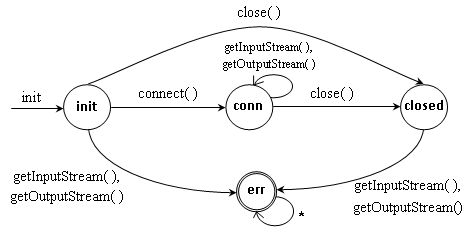
\includegraphics{./images/Fsa.png}
  \caption[FSA]{Partial typestate specification for java.net.Socket.}
  \label{fig:FSA}
\end{figure}


Figure 1.1  shows  a  finite state automaton providing a partial specification 
for the   java.net.SocketAPI. The finite state machine expresses the language of 
all program executions that violate this property. It monitors a connection's 
'close()', 'connect()' and 'getInputStream(),getOutputStream()' events and 
signals an error at its accepting state.\\\\
There are many typestate checking tools, both dynamic [4,7,8,13] and 
static[1,2,5,6], developed to ensure the correctness of property. While static 
program analysis inspect the program?Äôs code to prove the absence of typestate 
property violations for all possible executions of a given program, dynamic 
analysis tools incorporates a runtime monitor in the program under test that 
realizes the typestate properties that the program must satisfy. Testing all 
possible execution paths of complex systems endures high costs. Inorder to 
improve the
cost-effectiveness of static typestate analyses, researchers have combined 
multiple techniques [17, 18]. In [17], the authors present an intraprocedural 
analysis that eliminates the need for expensive whole-program analysis. The 
researchers have make use method annotations in the form of access permissions 
that specify typestate changes. [18] present a tool \textit{Plural} based on 
this approach and evaluate it using a few applications. Although impressive in 
many ways, these approaches still may produce false positives. Also, abnormal 
behaviour can be caused due to the deployment configurations and usage scenarios 
which cannot be examined by statically based testing techniques. \\As a result, 
dynamic analysis or runtime monitoring has gained considerable attention over 
static analysis. Researchers in runtime verification have developed powerful 
runtime monitoring tools [4,7,8,9,13]. These tools instrument the program under 
test with a runtime monitor and then, by composing the monitor with the program, 
the 
monitor observes the occurrence of each transition and decides whether the 
properties have been met or violated. Events are generated as a result of the 
instrumentation which keeps track of typestates. One important drawback of 
monitoring is that the instrumentation added to the program under test can yield 
significant overhead which hinders the monitoring of the application in 
practice. Depending on the program and property that are monitored, the overhead 
can vary significantly because the overhead depends on both the number of 
monitors that are created and the number of events generated during the program 
execution [14].\\\\
There have been several attempts earlier to optimise the runtime monitoring. 
[15, 16] present optimization techniques to reduce the overhead caused by the 
runtime overhead. They present techniques to remove unnecessary monitor 
instances. A number of hybrid techniques which combine static analysis and 
dynamic analysis to reduce the overhead have been proposed. In recent years the 
researchers[10, 12] have tried to apply the hybrid approach in which typestate 
property violation is first checked by static analysis to reduce the number of 
monitors at runtime monitoring. In [7], Arnold et al presents QVM that checks 
violations of correctness properties and has an overhead manager that enforces 
an overhead within limits. It is built on JVM so, comes with the cost of non 
portability.\\\\ 
In our research, we aim to create a framework based on sampling of objects for 
runtime monitoring that is deterministic and memory efficient. In our approach, 
we investigate the trade-off between the runtime overhead and the error 
reporting.  We are using a novel approach that works by limiting the number of 
monitors based on heuristics that are related to the program execution context. 
Depending on whether an object that is analysed has been previously monitored or 
not, the decision to sample the objects is made. In other words, monitoring will 
be performed only for the sampled objects to ensure that there is  redundancy 
among monitor's behavior of detecting the same error again and again. The total 
number of monitors generated for analysing the violations is restricted. In 
addition, the approach also limits the number of monitors that are associated 
with events related to a set of objects. Only a limited number of monitors are 
generated, thus utilizing memory efficiently. We have presented a cost model 
that aims to provide worst-case bounds for the execution times of handling 
events.\\\\
We implemented the sampled object based runtime monitoring framework on JavaMOP 
[4]. We used our framework to monitor two typestate properties, HasNext and 
UnsafeIterator, on some of the benchmarks from the Dacapo benchmark suite[11] 
and were able to capture the violations even after limiting the generation of 
monitors. We have also defined a cost model that gives the cost incurred in 
runtime monitoring by our approach to show that it is deterministic in terms of 
execution time.\\\\
\textbf{Outline} The rest of the report is as follows: Chapter 2 explains the 
motivation behind this research work. Chapter 3 provides a detailed overview of 
Sampled Object based Monitoring and shows an example. Chapter 4 presents the 
Cost Model of our approach. Chapter 5 presents our experimental data. Chapter 6 
discusses the related work. Chapter 7 provides some concluding remarks.
}